\documentclass[aps,prl,twocolumn,floatfix,letterpaper]{revtex4}

\usepackage{amsfonts}
\usepackage{amssymb}
\usepackage{amsthm}
\usepackage{amsmath,amscd}
\usepackage[all]{xy}
\usepackage{moreverb}
\usepackage{fancyhdr}
\usepackage[pdftex]{graphicx}

    \newtheorem{problem}{Problem}
    \newtheorem{theorem}{Theorem}[section]
    \newtheorem{lemma}[theorem]{Lemma}
    \newtheorem{proposition}[theorem]{Proposition}
    \newtheorem{corollary}[theorem]{Corollary}

    \newenvironment{solution}[1][Solution]{\begin{trivlist}
    \item[\hskip \labelsep {\bfseries #1}]}{\end{trivlist}}
    \newenvironment{definition}[1][Definition]{\begin{trivlist}
    \item[\hskip \labelsep {\bfseries #1}]}{\end{trivlist}}
    \newenvironment{example}[1][Example]{\begin{trivlist}
    \item[\hskip \labelsep {\bfseries #1}]}{\end{trivlist}}
    \newenvironment{remark}[1][Remark]{\begin{trivlist}
    \item[\hskip \labelsep {\bfseries #1}]}{\end{trivlist}}

  %  \newcommand{\qed}{\nobreak \ifvmode \relax \else
  %        \ifdim\lastskip<1.5em \hskip-\lastskip
  %        \hskip1.5em plus0em minus0.5em \fi \nobreak
  %        \vrule height0.75em width0.5em depth0.25em\fi}

    \renewcommand{\qedsymbol}{\textsquare}

\addtolength{\textwidth}{0.5in}
\addtolength{\hoffset}{-0.3in}
\addtolength{\textheight}{0.5in}
\addtolength{\voffset}{-0.3in}

\relpenalty=9999
\binoppenalty=9999

\newcommand{\PP}{\mathbb{P}}
\newcommand{\EE}{\mathbb{E}}
\newcommand{\FF}{\mathcal{F}}

\pagestyle{fancy}
%\fancyhead[CO,CE]{S.Chaichenets}
\fancyfoot[CO,CE]{S.Chaichenets}
\fancyfoot[RO, LE] {\thepage}


\begin{document}

\title{STAT 580 Stochastic Processes \\
	Assignment 5}
\author{ S.\ Chaichenets }
\date{\today}
\maketitle


%%%%%%%%%%%%%%%%%%%%%%%%%%%%%%%%%%%%%%%%%%%%

\begin{problem}
Probability space $\Omega := (-1,+1]$ with Lebesgue measure, random variable $X(\omega) := \omega^2$.
For $n=0,1,2,3,4$, define the $\sigma$-algebra
\begin{equation}
\FF_n := \sigma \left\{ \left( \frac{j}{2^n},\frac{j+1}{2^n}\right], j=-2^n,\ldots,2^n-1\right\}
\end{equation}
Sketch the graphs of the random variables $\EE(X|\FF_n)$.
\end{problem}

\begin{solution}
See appendix.
\qed
\end{solution}

\begin{problem}
Let $S_n : = X_0 + \ldots + X_n$ be a symmetric random walk on $\mathbb{Z}$; 
$\PP(X_i=-1) = \frac{1}{2} = \PP(X_i=+1)$.
The random variable $M_n := \frac{cos(S_n)}{cos^n(1)}$ is a martingale with respect to
$\FF_n := \sigma\left\{ X_0,\ldots,X_n\right\} $.
\end{problem}
\begin{solution}
We need to show that the following 3 properties hold:
\begin{enumerate}
	\item{$\EE(|M_n| < \infty \quad \forall n \geq 0$ \label{fini}}
	\item{$M_n\ {\rm is\ } \FF_n$ - adapted, $\forall n\geq0$ \label{adap1}}
	\item{$\EE(M_{n+1}|\FF_n) = M_n$ \label{exp1}}
\end{enumerate}
Property \ref{fini} follows from $ \left| \frac{cos(S_n)}{cos^n(1)}\right| 
		\leq \left| cos^{-n}(1) \right| 
		< \infty $;
property \ref{adap1} is by construction; and property \ref{exp1} is seen from
\scriptsize
\begin{equation}
\begin{split}
	\EE(cos(S_{n+1})|\FF_n) &= \frac{1}{2} (cos(S_n + 1) + cos(S_n - 1))		\\
		&= \frac{1}{2} (cos(S_n)cos(1) - sin(S_n)sin(1) 		\\
		& \qquad + cos(S_n)cos(1) + sin(S_n)sin(1))				\\
		&= cos(1) cos(S_n)
\end{split}
\end{equation}
\normalsize

\qed
\end{solution}

\begin{problem}
Let $(M_n)$ be a martingale with respect to $(\FF_n)$ and $T$ an $(\FF_n)$-stopping time with
$\PP(T<\infty) = 1$. Then $M_{T\wedge n}$ is also a martingale with respect to $(\FF_n)$.
\end{problem}
\begin{proof}
%For any $k\in \mathbb{N}$, and $T_k := T\wedge k$ be a bounded stopping time. 
%Then
$M_{T\wedge n}$ is $(\FF_n)$-adapted since 
$\FF_n \supseteq \FF_{n\wedge T}$.
Moreover, $M_{T \wedge n}$ is a $(\FF_n)$-martingale since
$$
\EE(M_{T \wedge n+1}|\FF_n) = \EE(M_{T\wedge n}|\FF_n)
$$
For	$n < T$	 because $M_n$  is a martingale, and 
	for $n \geq T$ because the process is stopped: $M_{T\wedge n} = M_{T}$
\end{proof}

\begin{problem}
Let $M_n := \sum_{j=0}^n \varepsilon_j/2^j$, where $\varepsilon_j$ are i.i.d with 
$\PP(\varepsilon_j = +1 ) = \frac{1}{2} = \PP(\varepsilon_j=-1)$. Run some fun simultions.
\end{problem}
\begin{solution}
15 sample paths, each 30 steps long, are plotted on Figure \ref{samplepaths} and show rather 
rapid convergence - which shouldn't be surprising since $M_n$ is absolutely convergent.
\begin{figure}
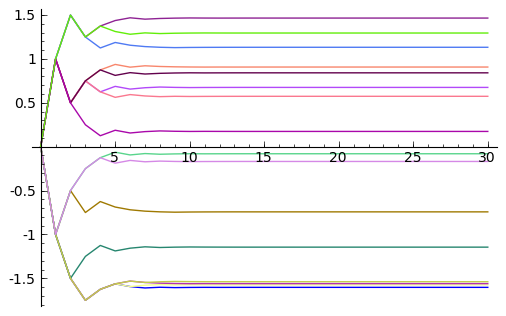
\includegraphics[height=.20\textheight]{hw5q4p1.png}
\caption[sample paths]
{sample paths}\label{samplepaths}
\end{figure}
Figure \ref{pdf} is collected from 8192 paths and indicates that $M_\infty$ is uniformly 
distributed on $[-2,+2]$ - this is is also not surprising.
%, and directly follows from the 
%fact $M_n$ is a martingale.
\begin{figure}
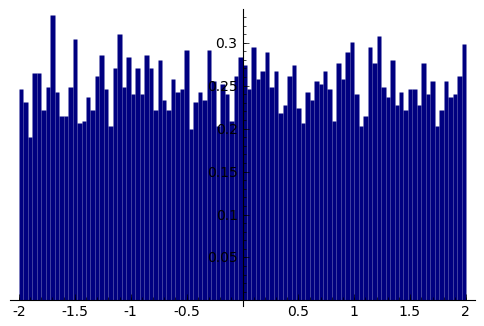
\includegraphics[height=.20\textheight]{hw5q4p2.png}
\caption[pdf]
{empirical pdf}\label{pdf}
\end{figure}
\qed
\end{solution}

\appendix
%\section*{Code Listing}
%
%scriptsize
%
%\normalsize
\end{document}

